\section{eo\-Es\-Global\-Xover$<$ EOT $>$ Class Template Reference}
\label{classeo_es_global_xover}\index{eoEsGlobalXover@{eoEsGlobalXover}}
Gloabl crossover operator for ES genotypes.  


{\tt \#include $<$eo\-Es\-Global\-Xover.h$>$}

Inheritance diagram for eo\-Es\-Global\-Xover$<$ EOT $>$::\begin{figure}[H]
\begin{center}
\leavevmode
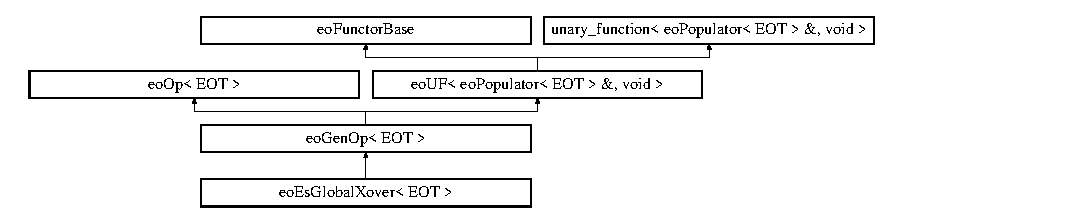
\includegraphics[height=2.54835cm]{classeo_es_global_xover}
\end{center}
\end{figure}
\subsection*{Public Types}
\begin{CompactItemize}
\item 
typedef EOT::Fitness {\bf Fit\-T}\label{classeo_es_global_xover_w0}

\end{CompactItemize}
\subsection*{Public Member Functions}
\begin{CompactItemize}
\item 
{\bf eo\-Es\-Global\-Xover} ({\bf eo\-Bin\-Op}$<$ double $>$ \&\_\-cross\-Obj, {\bf eo\-Bin\-Op}$<$ double $>$ \&\_\-cross\-Mut)\label{classeo_es_global_xover_a0}

\begin{CompactList}\small\item\em (Default) Constructor. \item\end{CompactList}\item 
virtual std::string {\bf class\-Name} () const \label{classeo_es_global_xover_a1}

\begin{CompactList}\small\item\em The class name. Used to display statistics. \item\end{CompactList}\item 
unsigned {\bf max\_\-production} (void)\label{classeo_es_global_xover_a2}

\begin{CompactList}\small\item\em The TOTAL number of offspring (here = nb of parents modified in place). \item\end{CompactList}\item 
void {\bf apply} ({\bf eo\-Populator}$<$ {\bf EOT} $>$ \&\_\-plop)
\begin{CompactList}\small\item\em modifies one parents in the populator using 2 new parents for each component! \item\end{CompactList}\end{CompactItemize}
\subsection*{Private Member Functions}
\begin{CompactItemize}
\item 
void {\bf cross\_\-self\_\-adapt} ({\bf eo\-Es\-Simple}$<$ Fit\-T $>$ \&\_\-parent, const {\bf eo\-Pop}$<$ {\bf eo\-Es\-Simple}$<$ Fit\-T $>$ $>$ \&\_\-pop)
\begin{CompactList}\small\item\em Method for cross self-adaptation parameters. \item\end{CompactList}\item 
void {\bf cross\_\-self\_\-adapt} ({\bf eo\-Es\-Stdev}$<$ Fit\-T $>$ \&\_\-parent, const {\bf eo\-Pop}$<$ {\bf eo\-Es\-Stdev}$<$ Fit\-T $>$ $>$ \&\_\-pop)
\begin{CompactList}\small\item\em Method for cross self-adaptation parameters. \item\end{CompactList}\item 
void {\bf cross\_\-self\_\-adapt} ({\bf eo\-Es\-Full}$<$ Fit\-T $>$ \&\_\-parent, const {\bf eo\-Pop}$<$ {\bf eo\-Es\-Full}$<$ Fit\-T $>$ $>$ \&\_\-pop)
\begin{CompactList}\small\item\em Method for cross self-adaptation parameters. \item\end{CompactList}\end{CompactItemize}
\subsection*{Private Attributes}
\begin{CompactItemize}
\item 
{\bf eo\-Random\-Select}$<$ {\bf EOT} $>$ {\bf sel}\label{classeo_es_global_xover_r0}

\item 
{\bf eo\-Bin\-Op}$<$ double $>$ \& {\bf cross\-Obj}\label{classeo_es_global_xover_r1}

\item 
{\bf eo\-Bin\-Op}$<$ double $>$ \& {\bf cross\-Mut}\label{classeo_es_global_xover_r2}

\end{CompactItemize}


\subsection{Detailed Description}
\subsubsection*{template$<$class EOT$>$ class eo\-Es\-Global\-Xover$<$ EOT $>$}

Gloabl crossover operator for ES genotypes. 

Uses some Atom crossovers to handle both the object variables and the mutation strategy parameters 



Definition at line 44 of file eo\-Es\-Global\-Xover.h.

\subsection{Member Function Documentation}
\index{eoEsGlobalXover@{eo\-Es\-Global\-Xover}!apply@{apply}}
\index{apply@{apply}!eoEsGlobalXover@{eo\-Es\-Global\-Xover}}
\subsubsection{\setlength{\rightskip}{0pt plus 5cm}template$<$class EOT$>$ void {\bf eo\-Es\-Global\-Xover}$<$ {\bf EOT} $>$::apply ({\bf eo\-Populator}$<$ {\bf EOT} $>$ \& {\em \_\-plop})\hspace{0.3cm}{\tt  [inline, virtual]}}\label{classeo_es_global_xover_a3}


modifies one parents in the populator using 2 new parents for each component! 

\begin{Desc}
\item[Parameters:]
\begin{description}
\item[{\em \_\-pop}]a POPULATOR (not a simple population) \end{description}
\end{Desc}


Implements {\bf eo\-Gen\-Op$<$ EOT $>$} {\rm (p.\,\pageref{classeo_gen_op_b0})}.

Definition at line 67 of file eo\-Es\-Global\-Xover.h.

References eo\-Es\-Global\-Xover$<$ EOT $>$::cross\_\-self\_\-adapt(), EO$<$ F $>$::invalidate(), and eo\-Populator$<$ EOT $>$::source().\index{eoEsGlobalXover@{eo\-Es\-Global\-Xover}!cross_self_adapt@{cross\_\-self\_\-adapt}}
\index{cross_self_adapt@{cross\_\-self\_\-adapt}!eoEsGlobalXover@{eo\-Es\-Global\-Xover}}
\subsubsection{\setlength{\rightskip}{0pt plus 5cm}template$<$class EOT$>$ void {\bf eo\-Es\-Global\-Xover}$<$ {\bf EOT} $>$::cross\_\-self\_\-adapt ({\bf eo\-Es\-Simple}$<$ Fit\-T $>$ \& {\em \_\-parent}, const {\bf eo\-Pop}$<$ {\bf eo\-Es\-Simple}$<$ Fit\-T $>$ $>$ \& {\em \_\-pop})\hspace{0.3cm}{\tt  [inline, private]}}\label{classeo_es_global_xover_d0}


Method for cross self-adaptation parameters. 

Specialization for {\bf eo\-Es\-Simple}{\rm (p.\,\pageref{classeo_es_simple})}. 

Definition at line 94 of file eo\-Es\-Global\-Xover.h.

References eo\-Es\-Simple$<$ Fit $>$::stdev.

Referenced by eo\-Es\-Global\-Xover$<$ EOT $>$::apply().\index{eoEsGlobalXover@{eo\-Es\-Global\-Xover}!cross_self_adapt@{cross\_\-self\_\-adapt}}
\index{cross_self_adapt@{cross\_\-self\_\-adapt}!eoEsGlobalXover@{eo\-Es\-Global\-Xover}}
\subsubsection{\setlength{\rightskip}{0pt plus 5cm}template$<$class EOT$>$ void {\bf eo\-Es\-Global\-Xover}$<$ {\bf EOT} $>$::cross\_\-self\_\-adapt ({\bf eo\-Es\-Stdev}$<$ Fit\-T $>$ \& {\em \_\-parent}, const {\bf eo\-Pop}$<$ {\bf eo\-Es\-Stdev}$<$ Fit\-T $>$ $>$ \& {\em \_\-pop})\hspace{0.3cm}{\tt  [inline, private]}}\label{classeo_es_global_xover_d1}


Method for cross self-adaptation parameters. 

Specialization for {\bf eo\-Es\-Stdev}{\rm (p.\,\pageref{classeo_es_stdev})}. 

Definition at line 106 of file eo\-Es\-Global\-Xover.h.

References eo\-Es\-Stdev$<$ Fit $>$::stdevs.\index{eoEsGlobalXover@{eo\-Es\-Global\-Xover}!cross_self_adapt@{cross\_\-self\_\-adapt}}
\index{cross_self_adapt@{cross\_\-self\_\-adapt}!eoEsGlobalXover@{eo\-Es\-Global\-Xover}}
\subsubsection{\setlength{\rightskip}{0pt plus 5cm}template$<$class EOT$>$ void {\bf eo\-Es\-Global\-Xover}$<$ {\bf EOT} $>$::cross\_\-self\_\-adapt ({\bf eo\-Es\-Full}$<$ Fit\-T $>$ \& {\em \_\-parent}, const {\bf eo\-Pop}$<$ {\bf eo\-Es\-Full}$<$ Fit\-T $>$ $>$ \& {\em \_\-pop})\hspace{0.3cm}{\tt  [inline, private]}}\label{classeo_es_global_xover_d2}


Method for cross self-adaptation parameters. 

Specialization for {\bf eo\-Es\-Full}{\rm (p.\,\pageref{classeo_es_full})}. 

Definition at line 121 of file eo\-Es\-Global\-Xover.h.

References eo\-Es\-Full$<$ Fit $>$::correlations, and eo\-Es\-Full$<$ Fit $>$::stdevs.

The documentation for this class was generated from the following file:\begin{CompactItemize}
\item 
eo\-Es\-Global\-Xover.h\end{CompactItemize}
